\section{\name for IO Integity}
\label{sec:systemDesign}


In this section, we provide the technical details of \name integrity protection for IO devices. 

\myparagraph{\device setup} We assume that the \device manufacturer issues a certificate for each of the deployed \device{}s . The \device maintains a whitelist for the remote servers along with their public certificates. This allows the \device to verify messages signed by those remote servers. It is also possible to establish a conventional \tls channel between the \device and the server using the HDMI signal as downstream channel and keystrokes from the \device as the upload channel. Note that IO integrity does not require a \tls between the \device and the remote server. Such a \tls channel is strictly necessary to provide IO confidentiality that is discussed later in Section~\ref{sec:confidentiality}.  For now, we only focus on IO integrity in this section.


\begin{figure*}[t]
\centering
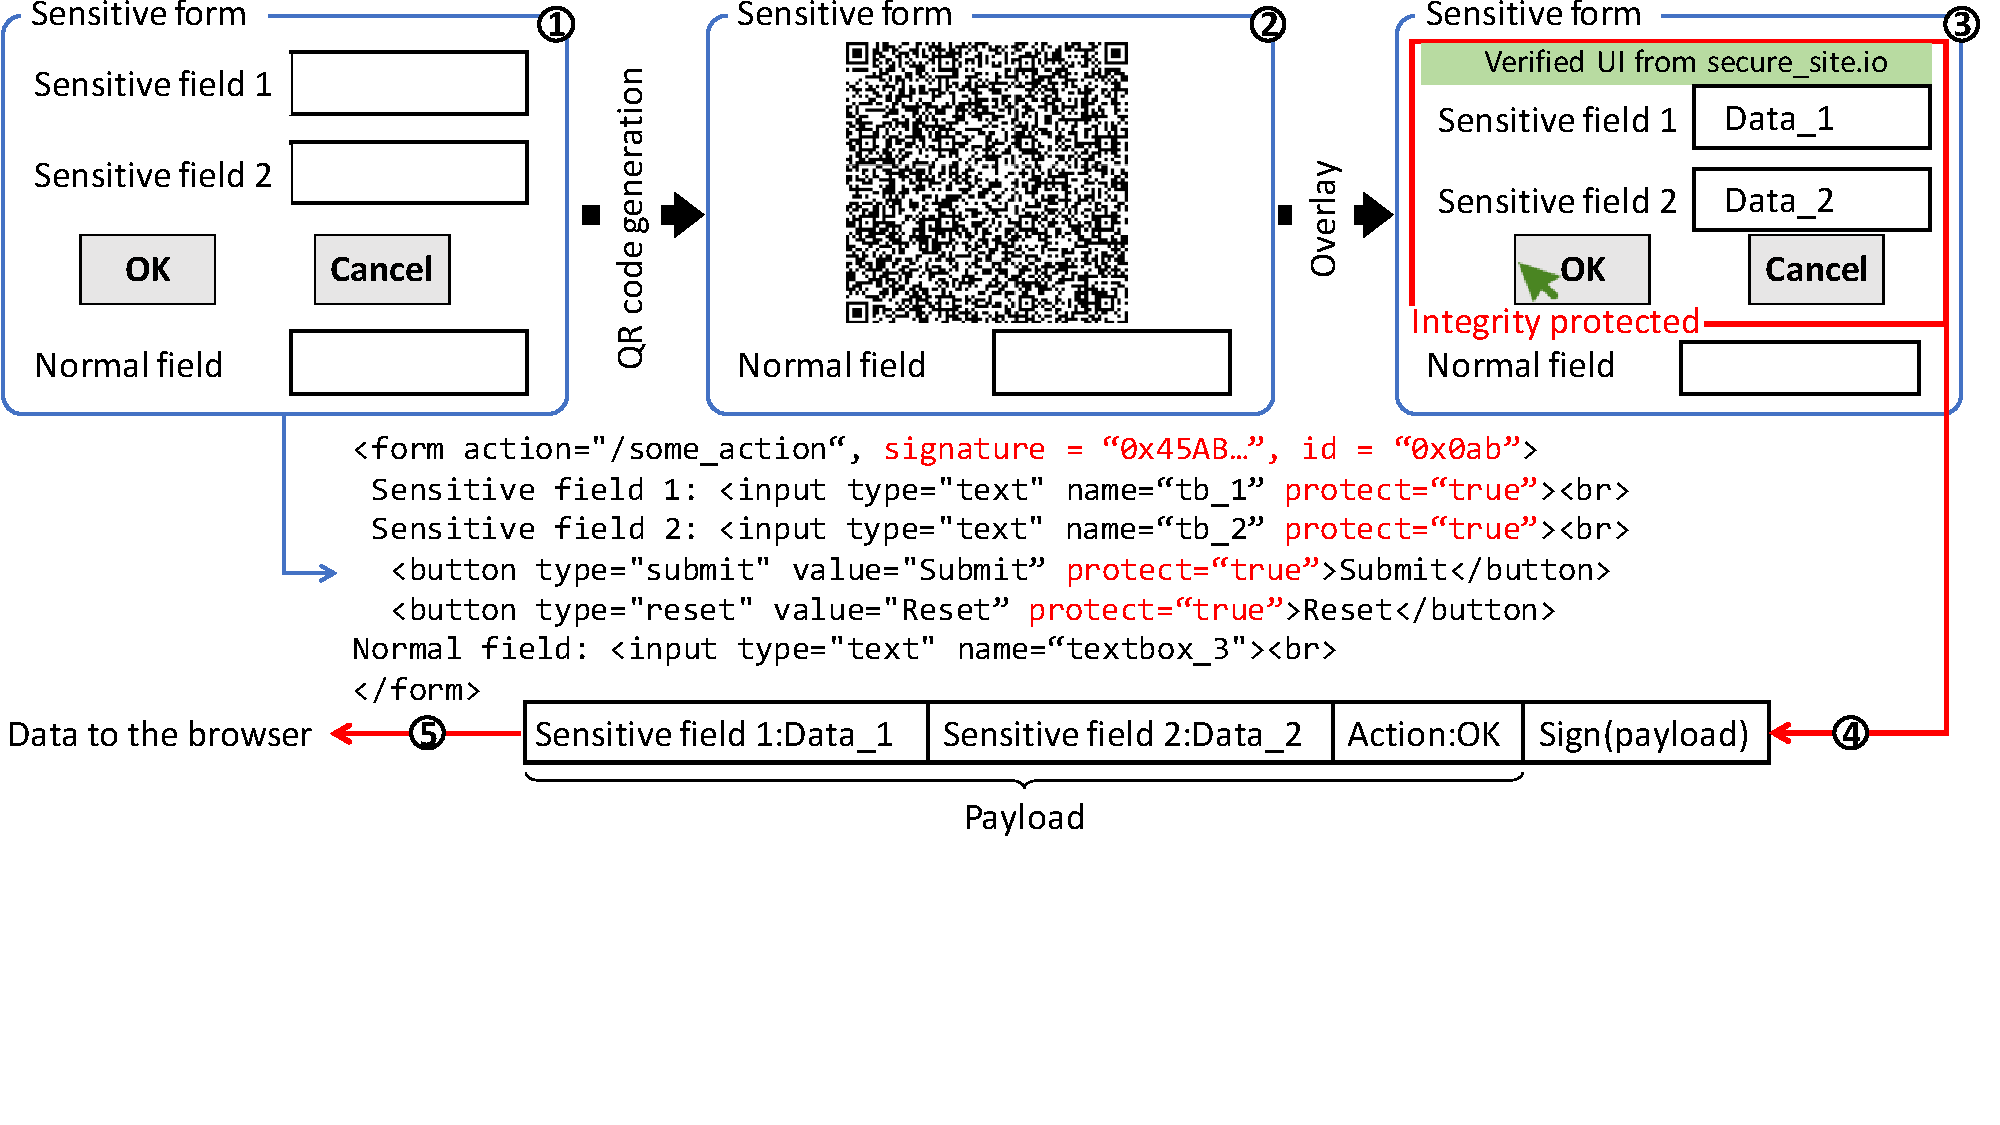
\includegraphics[trim={0 4.8cm 0 0}, clip, width=0.8\linewidth]{formTransform.pdf}
%\caption{\textbf{Transformation of UI elements: UI $\rightarrow$ QR code $\rightarrow$ \device generated UI overlay.} Automated transformation of the UI elements (\one) by the \name JavaScript snippets that detects the presence of the device. The corresponding \html source shows the UI elements that require integrity/privacy protection. These UI elements are transformed into a QR code (\two). The QR code encodes a UI specification that recreates the transformed UI. Specification~\ref{snippet:UISpecification} shows the corresponding UI specification that is created by the \name \js code. The QR code is then decoded and overlaid (\three) on the HDMI stream by the \device. Upon the user's action on the overlaid UI elements, the device signs all the input data and send them to the remote server. As the rendered UI is generated and overlaid by the \device, it also ensures the integrity of the UI elements. Note that the intermediate QR code transformation (\two) is not visible by the user as it is decoded instantaneously by the device.}
\caption{\textbf{Transformation of UI elements: UI $\rightarrow$ encoded specification $\rightarrow$ \device generated UI overlay.} \one The actual webpage and the corresponding \html source shows the UI elements that requires integrity protection. \two These UI elements are transformed into an encoded UI specification (our \name prototype uses QR code that encodes a UI specification, e.g., Specification~\ref{snippet:UISpecification}) by the \name JS. The QR code. \three AThe QR code decoded and overlaid on the HDMI stream by the \device. \four Upon the user's action on the overlaid UI elements, the device signs all the input data. \five The \device sends these signed input data them to the remote server. Note that the intermediate QR code transformation (\two) is not visible by the user as it is decoded instantaneously by the device.}
\spacesave
\label{fig:transformation}
\end{figure*}


\subsection{\device Overlay of UI Elements}
\label{sec:systemDesign:transformation}

%As we have seen in the strawman solution described in Section~\ref{sec:approach:strawman}, taking a screenshot or capturing a video of the screen that the user is viewing to ensure IO integrity is impractical in the real world.
As we discussed in the previous sections, both output and input integrity are needed to be protected in order to achieve any one of them. \name ensures output integrity by isolating a part of the display that can be ovserved and modified by the attacker controlled host. \device intercepts the HDMI signal from the untrusted host and inject overlay bitmaps of sensitive UI on the screen. The overlay mechanism provides output integrity, which in turn ensures the input integrity as the attacker can not draw on top of the \device-generated overlay to trick the user into providing incorrect input. Note that as illustrated in Figure~\ref{fig:screenshot_1}, the \device only overlays on a small part of the screen that contains sensitive information and takes
security-critical inputs from the user.

%\subsubsection{\bfseries \device generated UI overlay} \label{sec:systemDesign:transformation:overlay}
 
This approach requires a JavaScript code snippet that we call \name JS, that executes on the host. The \name JS snippet that is served with the webpage transforms the UI elements that require IO integrity protection. Note that \name JS runs on the browser and is not trusted in our system model. We illustrate the method of UI transformation in Figure~\ref{fig:transformation}. The entire process has two phases: (i) UI $\rightarrow$ encoded specification generation, and (ii) Encoded specification $\rightarrow$ Overlay.


\begin{mylist}
\item \textbf{UI $\rightarrow$ encoded specification generation.} In our implementation of \name, we use the QR code as the intermediate representation of the UI elements that the \name JS generates and the \device interprets. The developers annotates the sensitive UIs in the HTML source (as \texttt{protect=``true''}) that the \name \js parses and convert to a intermediate representation that \device understands. The idea is similar to the developer's annotation if security-critical UIs that is recommended in W3C UI security policy~\cite{w3c_spec}. Note that \name is agnostic of the type of intermediate representation. We use the QR code as it is efficient and can be represented as an image in the HDMI stream that the \device intercepts. Figure~\ref{fig:transformation} shows this transformation between the step \one and \two. The \name JS also attaches the digital signature of the generated specification (\texttt{signature} attribute in the \texttt{form}). The server generates this signature by generating the specification statically from the webpage. \name \js then encodes this specification into a QR code and attaches it into the \texttt{dom} tree of the webpage. Note that the user never sees the QR code as it gets decoded and overlaid by the \device. The UI specification describes the UI elements that the \device interprets and uses to generate the UI bitmap that is used for the overlay. One such concrete example of the UI specification is provided in Specification~\ref{snippet:UISpecification}. Section~\ref{sec:prototype:impl:qr} provides detailed implementation details of how the \name JS generates the encoded UI specification. 

\item \textbf{Encoded specification $\rightarrow$ Overlay.} Overlay is the next phase where the encoded specification (QR code) that embeds the UI specification is interpreted by the \device and overlaid on the HDMI stream. The overlay faithfully recreates the UI to prevent any alteration in the user experience. The \device overlay is depicted in \three in Figure~\ref{fig:transformation}. The \device come with a small interpreter routine that converts the UI specifications to bitmaps that are then overlaid on the HDMI stream. The specification also contains the location and the size details (omitted from the Specification~\ref{snippet:UISpecification}). The \device uses this information to determine the specific UI element over which the user has her mouse pointer. As the \device parses all the HDMI frames for the QR code, the overlay does not get interrupted by scrolling. As the specification sent by the server is signed (\texttt{signature} attribute in the UI specification mentioned in the Specification~\ref{snippet:UISpecification}), the \device-generated UI overlay ensures the integrity and the authenticity of the UI elements on the web page. Note that the \device always draws on top of the frames that are rendered by the compromised host. This way, the overlaid UI is always visible by the user on display, and the host can not manipulate the overlays. Hence \emph{output integrity} is ensured.

\end{mylist}

%\subsubsection{\bfseries Integrity of the UI elements}

%Output integrity ensures the integrity of the UI elements that are sent by the remote server. 

%\subsubsection{Integrity of the user input} After the UI elements are correctly overlaid on the screen, the users can interact with these UI elements. The user interaction with the overlaid UI element is no different than a standard UI, making the user habituation seamless. The UI specification encodes the behavior of all the generated UI elements, making the \device aware of the semantics of the UI objects. E.g., when a user selects a text box and types on her keyboard, the \device intercepts all the keyboard strokes and overlays the characters on the UI. When the user clicks on the \texttt{OK} button on the overlay, the device gathers all the intercepted keyboard and mouse events, signs them and send them to the remote server. One example of the proof-of-action is depicted in Figure~\ref{fig:transformation} that shows the payload that the \device sends to the server. Along with the keyboard data that is provided by the user, the \device also attaches the proof that the user indeed clicked on the \texttt{OK} button that leads to the action. A detailed description of how the input is recorded and committed is presented in Section~\ref{sec:systemDesign:commit}.


\subsection{Focusing User Attention}
\label{sec:systemDesign:userAttention}

In the previous sections, we provide mechanisms to provide output integrity. Note that the output integrity is crucial to ensure input integrity as the untrusted host may show arbitrary information to the user (via the untrusted part of the display space) that may influence the user. Hence, it is necessary for \name to provide a visual cue to the user so that they can distinguish the secure overlay of the screen from the insecure part of the screen. There are two aspects of UI manipulation by the attacker-controlled host. i) spacial: where the attacker uses the non-overlaid part of the screen to influence the user, and ii) temporal: where the attacker may influence the user previously (in different webpage or application before) that leads to change of user input.

\myparagraph{Our solution} There exist several techniques in the context of browser-based security that can be used to focus user attention to the sensitive UI elements. Two of such well-known techniques are lightbox and freezing~\cite{huang2012clickjacking}. Lightbox dims out non-overlaid part of the screen (all the screen area excluding the overlaid mouse pointer and the overlaid UI). While freezing mechanism stalls all the visual activities on the display frame when the user enters into the overlaid UI. There exist other ways to grab user attention, but we omit them as those rely on other output channels such as sound etc. The developers can mention which mechanism to the user in the HTML. By default, \name applies lightbox in case no focusing mechanism is mentioned. There are two ways to activate these mechanisms: automatic and secure attention sequence (SAS). Both have their pros and cons.


\subsubsection{\bfseries Automated activation}
\label{sec:systemDesign:userAttention:automated}

This method can be triggered (dimming out or freezing the non-overlaid part of the screen) automatically in specific situations, e.g., when the user moves her mouse pointer over the overlaid UI, or start moving the mouse after a brief pause (like 5 seconds). One advantage of the automated trigger is that the user does not need to remember to trigger the mechanism. Hence the system is resilient from the situation where the user needs to trigger it. However, dimming out a large portion of the scene frequently can diminish user experience significantly.   

\subsubsection{\bfseries Secure Attention Sequence}
\label{sec:systemDesign:userAttention:sas}

Secure Attention Sequence (SAS) is a sequence of actions\footnote{Such as keystrokes \texttt{Ctrl+Alt+Del} that allows the user to provide her credential.} executed by the user that is completely trustworthy. SAS prevents an untrusted system from triggering an event that is otherwise sensitive to the user. Note that SAS is a well-researched topic in the context of UI/UX design. \name uses off-the-shelf SAS mechanism that provides a visual aid for the user to distinguish overlaid UI and the mouse pointer location and adapts it into the system. 

\myparagraph{SAS policy} The remote server can set configurable SAS policy per overlaid UI (i.e., QR code). The SAS policy is defined in the \texttt{SAS} attribute in the example specification provided in Specification~\ref{snippet:UISpecification}. By default, the overlaid UI is locked from the user and requires a key press from the user to unlock the sensitive UI. This information is overlaid on the UI to remind the user to execute this. One example policy could be \texttt{Ctrl+d:5}, which denotes that the user needs to press key `\texttt{Ctrl+d}' to unlock the UI overlay. Pressing this key also trigger the \device to back out the HDMI frames except for the UI overlay and the mouse pointer overlay for a specified time (here for $5$ seconds). 

\subsection{Continuous Tracking of Mouse Pointer in the HDMI Frame}
\label{sec:systemDesign:analysis}


\begin{figure}[t]
\centering
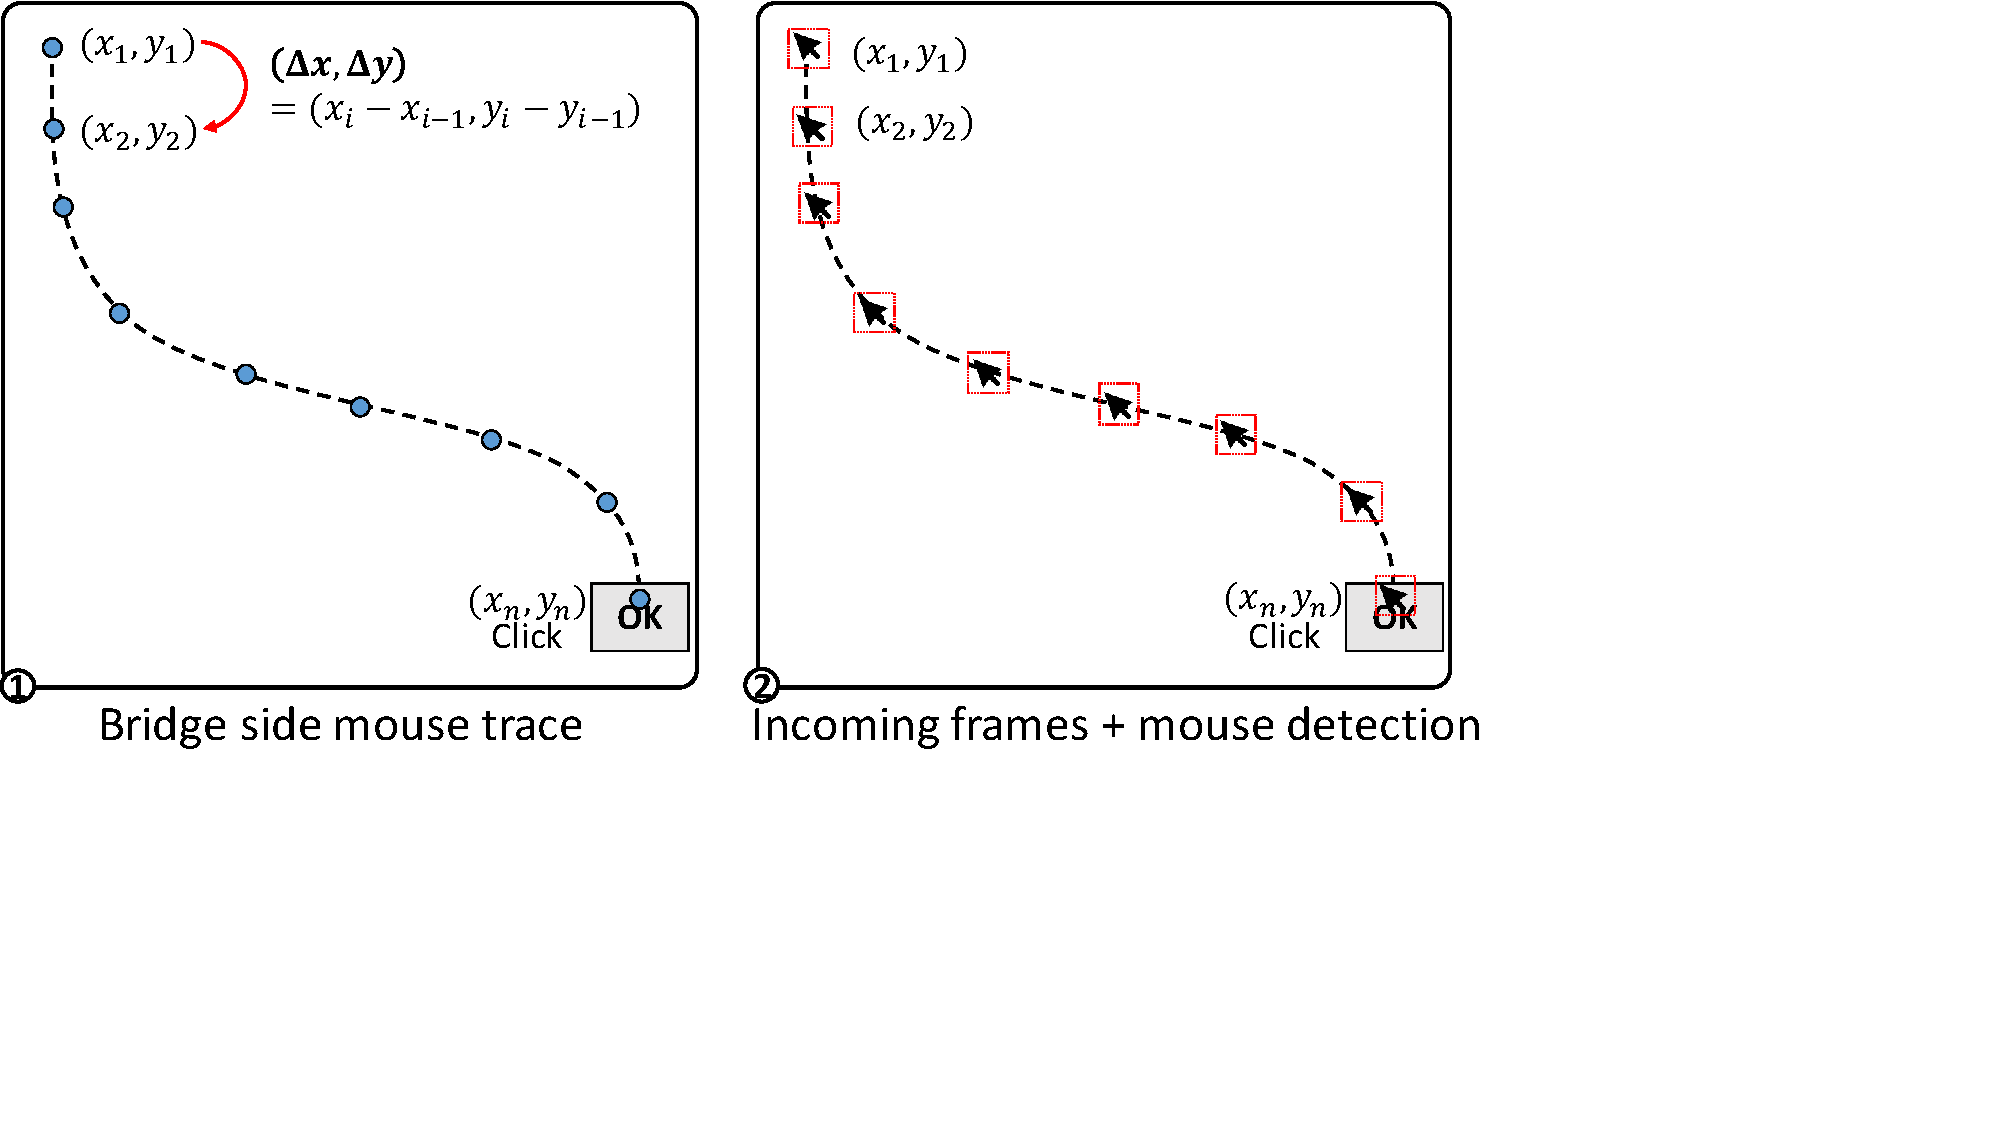
\includegraphics[trim={0 5.8cm 8cm 0}, clip, width=\linewidth]{mouseAnalysis.pdf}
\caption{\textbf{Pointer tracking.} \one The \device captures the raw mouse events ($\Delta x, \Delta y$) from the mouse that is attached to the \device. \two The \device captures the frames from the HDMI channel and checks into the designated pixel position $(x_i + \Delta x, y_i + \Delta y)$ if there exists a pointer. $t_1, t_2,\ldots t_n$ are the time instances when the \device receives the mouse data. $f_1, f_2,\ldots f_n$ are the corresponding HDMI frames that the \device intercepts.}
\spacesave
\label{fig:mouseAnalysis}
\centering
\end{figure}


In the previous section, we discuss how to focus user attention to isolate the overlaid part of the screen from the non-overlaid part of the screen. The focusing mechanisms rely on the user's mouse movement on the screen as entering the overlay triggers the focusing mechanisms. The triggering mechanisms pose a significant challenge to us as the \device does not know the current position of the mouse cursor on display. As the host is attacker-controlled, we cannot rely on the host to communicate the mouse position reliably to the \device. To address this, \name continuously tracks the current mouse cursor position from the HDMI frame (using shape detection) as it has access to both the HDMI channel and the raw mouse data.
Moreover, the host's pointer cannot be visible when the user interacts with the overlay rendered by the \device as the \device always draws on top of the HDMI frames. The \device intercepts the HDMI frames and mouse signals to 1) extract the mouse pointer and correlate it with the mouse data and 2) overlay a mouse pointer that is prominent and easy to follow. The pointer tracking and the overlay address three major challenges: i) both the \device and the user have the same sense of the mouse, ii) the \device precisely knows when to trigger the focusing mechanisms, and iii) the user can interact with the overlaid UI seamlessly. 


\subsubsection{\bfseries Calibration}\label{sec:systemDesign:analysis:calibration} When the user connects the \device for the first time after booting up, the \device performs an automated calibration to find the pointer. The \device gives very high mouse movement values that push the mouse pointer to the top-right corner of the screen. Then the \device tries to find the pointer there from the HDMI frames. If the \device is successful into finding the mouse pointer there, it continues tracking the pointer after that. Note, that at any point, if the \device loses track of the mouse pointer, the user can recalibrate it by reinitializing the \device.

\subsubsection{\bfseries Detection of pointer} The \device ensures pointer integrity by tracking the mouse movements using the HDMI frames and the raw mouse data. Figure~\ref{fig:mouseAnalysis} illustrates the high-level idea: 

\begin{mylist}
\item[]\one shows raw mouse data that sends the displacements $(\Delta x, \Delta y)$ over $x$ and $y$ axis that we over time series $t_1,\ldots, t_n$. Note that the initial mouse position is known to the \device from pointer calibration (refer to Section~\ref{sec:systemDesign:analysis:calibration}) where $(x_0, y_0) = (0, 0)$.  
\item[]\two shows the HDMI frames $f_1,\ldots f_n$ where the \device expects the mouse pointer to be found. For efficiency, the \device only scans over a small portion of the HDMI frames ($50 \times 50$ square pixels) that is enough to cover a mouse pointer. \device checks if there exists a mouse inside this square or not. In case there exists a mouse cursor, the \device allows further user interactions; otherwise, it stops all the communications and shows an error on display
\end{mylist}


\subsubsection{\bfseries Overlay of the mouse pointer} The \device draws a mouse pointer that is visible by the user. The overlaid mouse pointer is on top of the host rendered mouse pointer. The overlay provides a telltale sign to the user about the location of the mouse pointer in the case the host renders other mouse pointers on the screen to confuse the user. To emphasize the location of the mouse pointer, the \device highlights the overlaid pointer by dimming out the rest of the screen when there is a threshold time break (i.e., no input coming from the user for around 3 seconds). Note that as long as the \device is connected to the host, it always detect and overlay the mouse pointer irrespective of the application that is running on the host. In Section~\ref{sec:securityAnalysis:integrity} we provide the security analysis of the mouse pointer tracking and the overlay mechanism.


\subsubsection{\bfseries Coping with the disappearing cursor} Many OS offers a feature where the mouse pointer disappear from the screen when the user types in a text editor/browser. When the user moves her mouse again, the cursor again appears at the same position from where it was disappeared in the first place. From the \device's perspective, it is hard to distinguish between this case and the attacker deliberately removing the mouse pointer from the screen. To handle the case where the mouse pointer disappears from the screen when the user starts typing, the \device listens to all the keyboard input as the keyboard is also connected to the \device. When the \device detects there are keystrokes, it expects the cursor to be disappeared from the screen. When the \device again starts receiving input from the mouse, it checks if the cursor appears again on the screen at the exact location from where it disappeared - this way the \device ensures the consistency of the pointer position.  


\subsubsection{\bfseries Handling different mouse cursors} The \device is preloaded with the template images of the mouse cursor for identification. For our \name prototype implementation, we use the default cursors provided by the Ubuntu OS. This allows the \device to identify the cursor when it changes on the screen, e.g., from pointer to a hand when the user hovers her mouse over a link on the browser. 

 

\subsection{Protected User Interaction}
\label{sec:systemDesign:commit}

When the user finishes providing her input via input devices (mouse and keyboard), the \device sends these values (with signature to ensure integrity) to the remote server. Sending these signed input values to the server requires an upstream channel from the \device to the server.

\subsubsection{\bfseries Upstream channel}\label{sec:systemDesign:commit:upload} The data from the \device to the remote server is transmitted using the \name JavaScript snippet that is served by the remote web server. The \name JavaScript snippet uses a hidden text field to accept data coming from the \device. The \device emulates itself as a composite human interface device (HID) when it is connected to the host. The \device emulates keystrokes that transmit encoded data to the \name JavaScript snippet that is sent to the remote server via \texttt{XMLHttpRequest} call.

\subsubsection{\bfseries Sending input data}\label{sec:systemDesign:commit:send}
The user input transmission procedure is illustrated in Figure~\ref{fig:transformation}. This has two phases: \emph{record} and \emph{transmit} as described in the following:

\begin{mylist}
\item \textbf{Record.} After the UI elements are correctly overlaid on the screen, the users can interact with these UI elements. The user interaction with the overlaid UI element is no different than a standard UI. The UI specification encodes the behavior of all the generated UI elements, making the \device aware of the semantics of the UI objects. E.g., when a user selects a text box and types on her keyboard, the \device intercepts all the keyboard strokes and overlays the characters on the UI.
When user enters input data in the rendered overlay UI elements (such as textbox, button, slider, radio button, etc.), the \device records that in a (key, value) pair where the key is the identifier of the UI element (\texttt{id} in Specification~\ref{snippet:UISpecification}) and the value is the user provided value. The \texttt{type} of the UI elements determine what information to record. For example, the \device records all the keystrokes when a textbox is selected, the value corresponding to the position of the slider is recorded when the user interacts with a slider, etc. One example of the recording of the input data corresponding to the UI illustrated in Figure~\ref{fig:transformation} and Specification~\ref{snippet:UISpecification} is: 
\begin{align*}
Record = & (textbox\_1, Data\_1);(textbox\_2,Data\_2)
\end{align*}

\item \textbf{Transmit.} In the transmit phase, the \device waits for the user to select UI element which has a \texttt{trigger} capability (see Section~\ref{sec:systemDesign:transformation}).  When user clicks the \texttt{OK} button, the device signs the record. One such signed packet is also illustrated in Figure~\ref{fig:transformation}. Using the upstream channel (see Section~\ref{sec:systemDesign:commit:upload}), the \device sends the signed packet to the remote server.
\end{mylist} 

\subsubsection{\bfseries Server-side verification} \label{sec:systemDesign:commit:verification}Upon receiving the signed input data from \device, the remote accepts the input if the signature verification is successful. Note, if an input field is annotated as \texttt{protect=``true''}, the server does not accept any input without the \device signature. This prevents the attacker-controlled host to submit data. 

\subsubsection{\bfseries Changing browser tabs or browsers}
The \device supports multiple browsing tabs across multiple browsers. The UI specification contains \texttt{formId} and \texttt{domain} that works as the unique identifier for a specific form served from a specific web server. The \device can maintain multiple parallel TLS connection to web servers. Depending on the observed \texttt{formId} and \texttt{domain} (refer to Specification~\ref{snippet:UISpecification}), the device retrieved the data that is entered by the user. This way even if the user switches tabs, the \device can still allow editing the forms across tabs.


\subsection{Sequence of Events}
\label{sec:systemDesign:mainProtocol}

\iffalse
\begin{figure}[t]
\centering
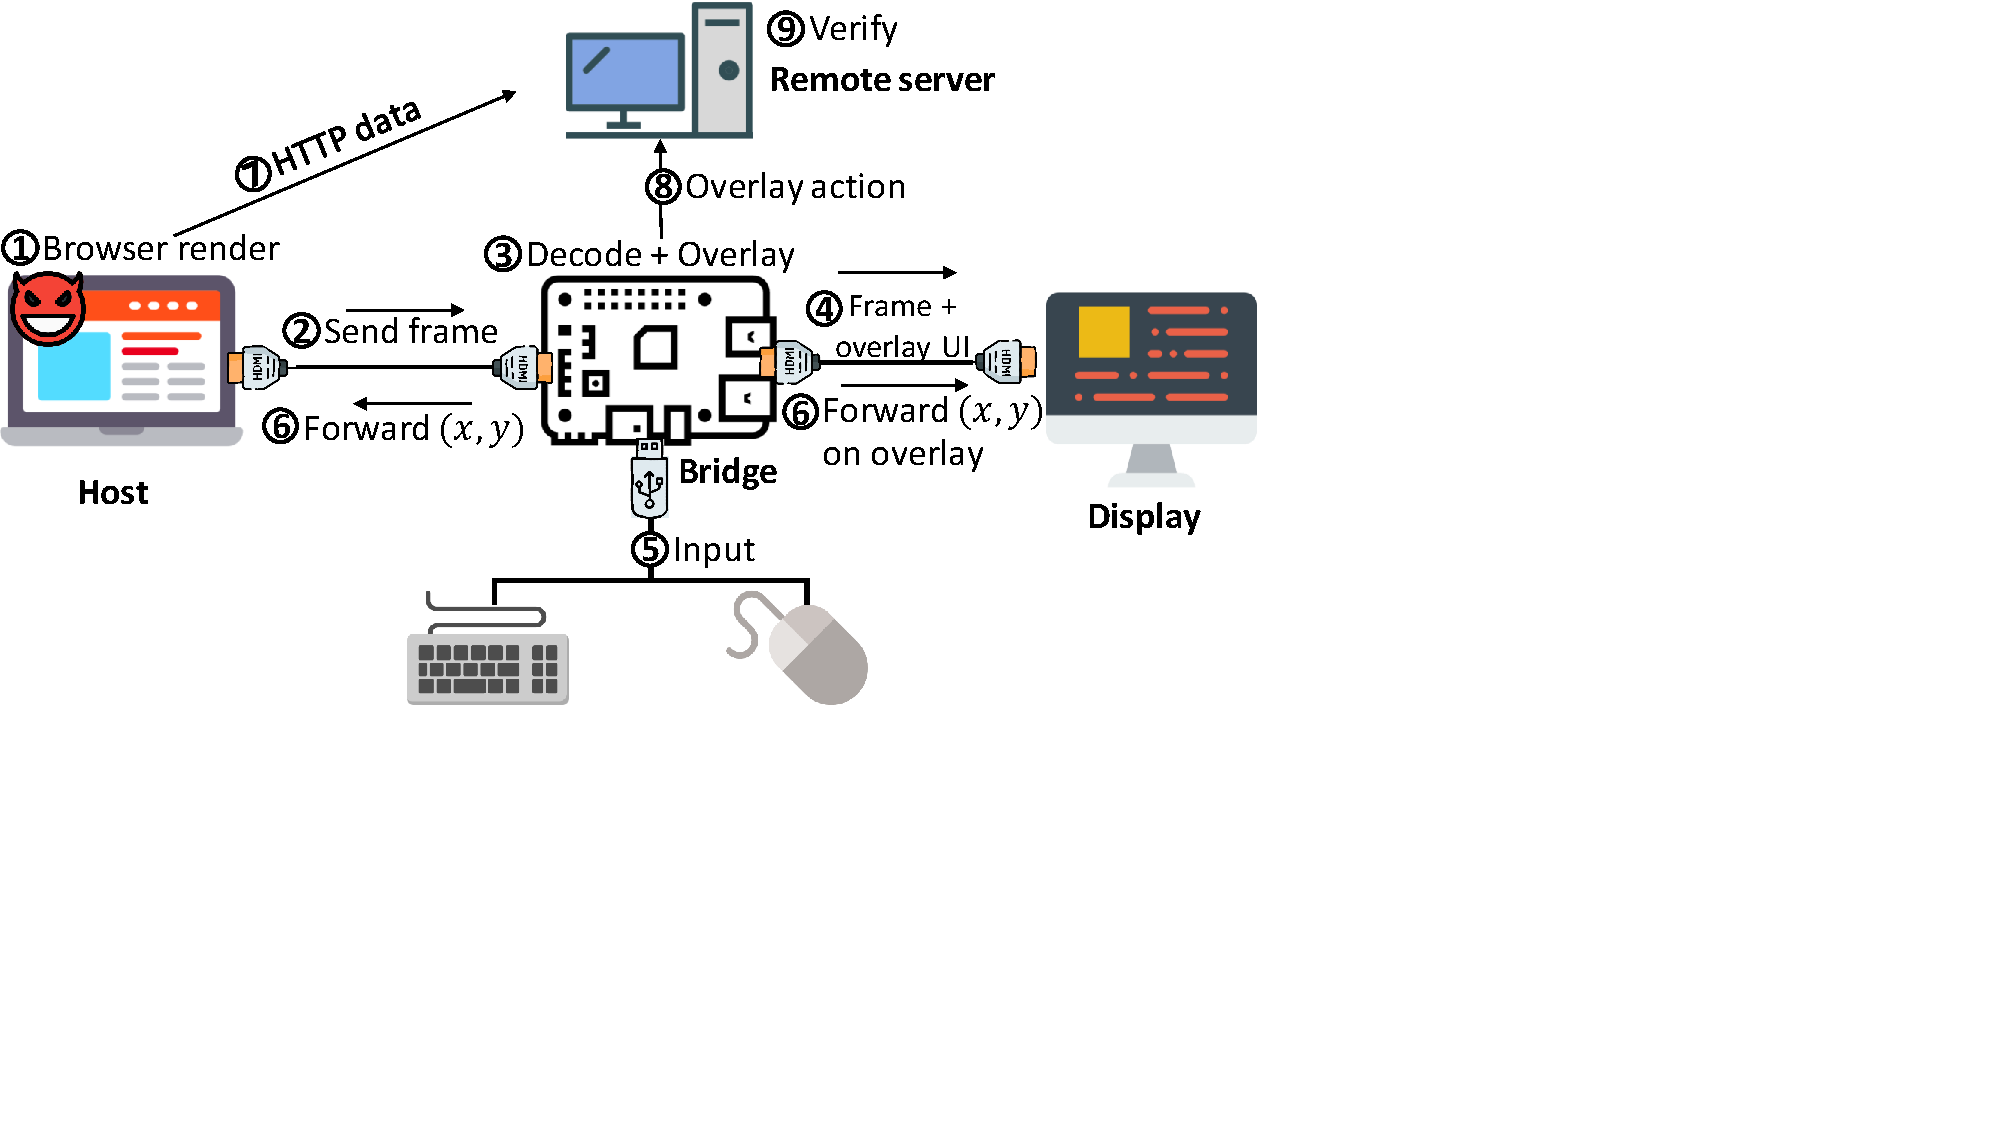
\includegraphics[trim={0 6.5cm 12cm 0}, clip, width=\linewidth]{systemDesign.pdf}
\caption{\textbf{Flow of the \name main protocol.} The figure shows the high-level protocol flow and the main messages that are exchanged between the remote server, host, \device, and the Io devices.}
\spacesave
\label{fig:systemDesign}
\centering
\end{figure}
\fi

\begin{figure}[t]
\centering
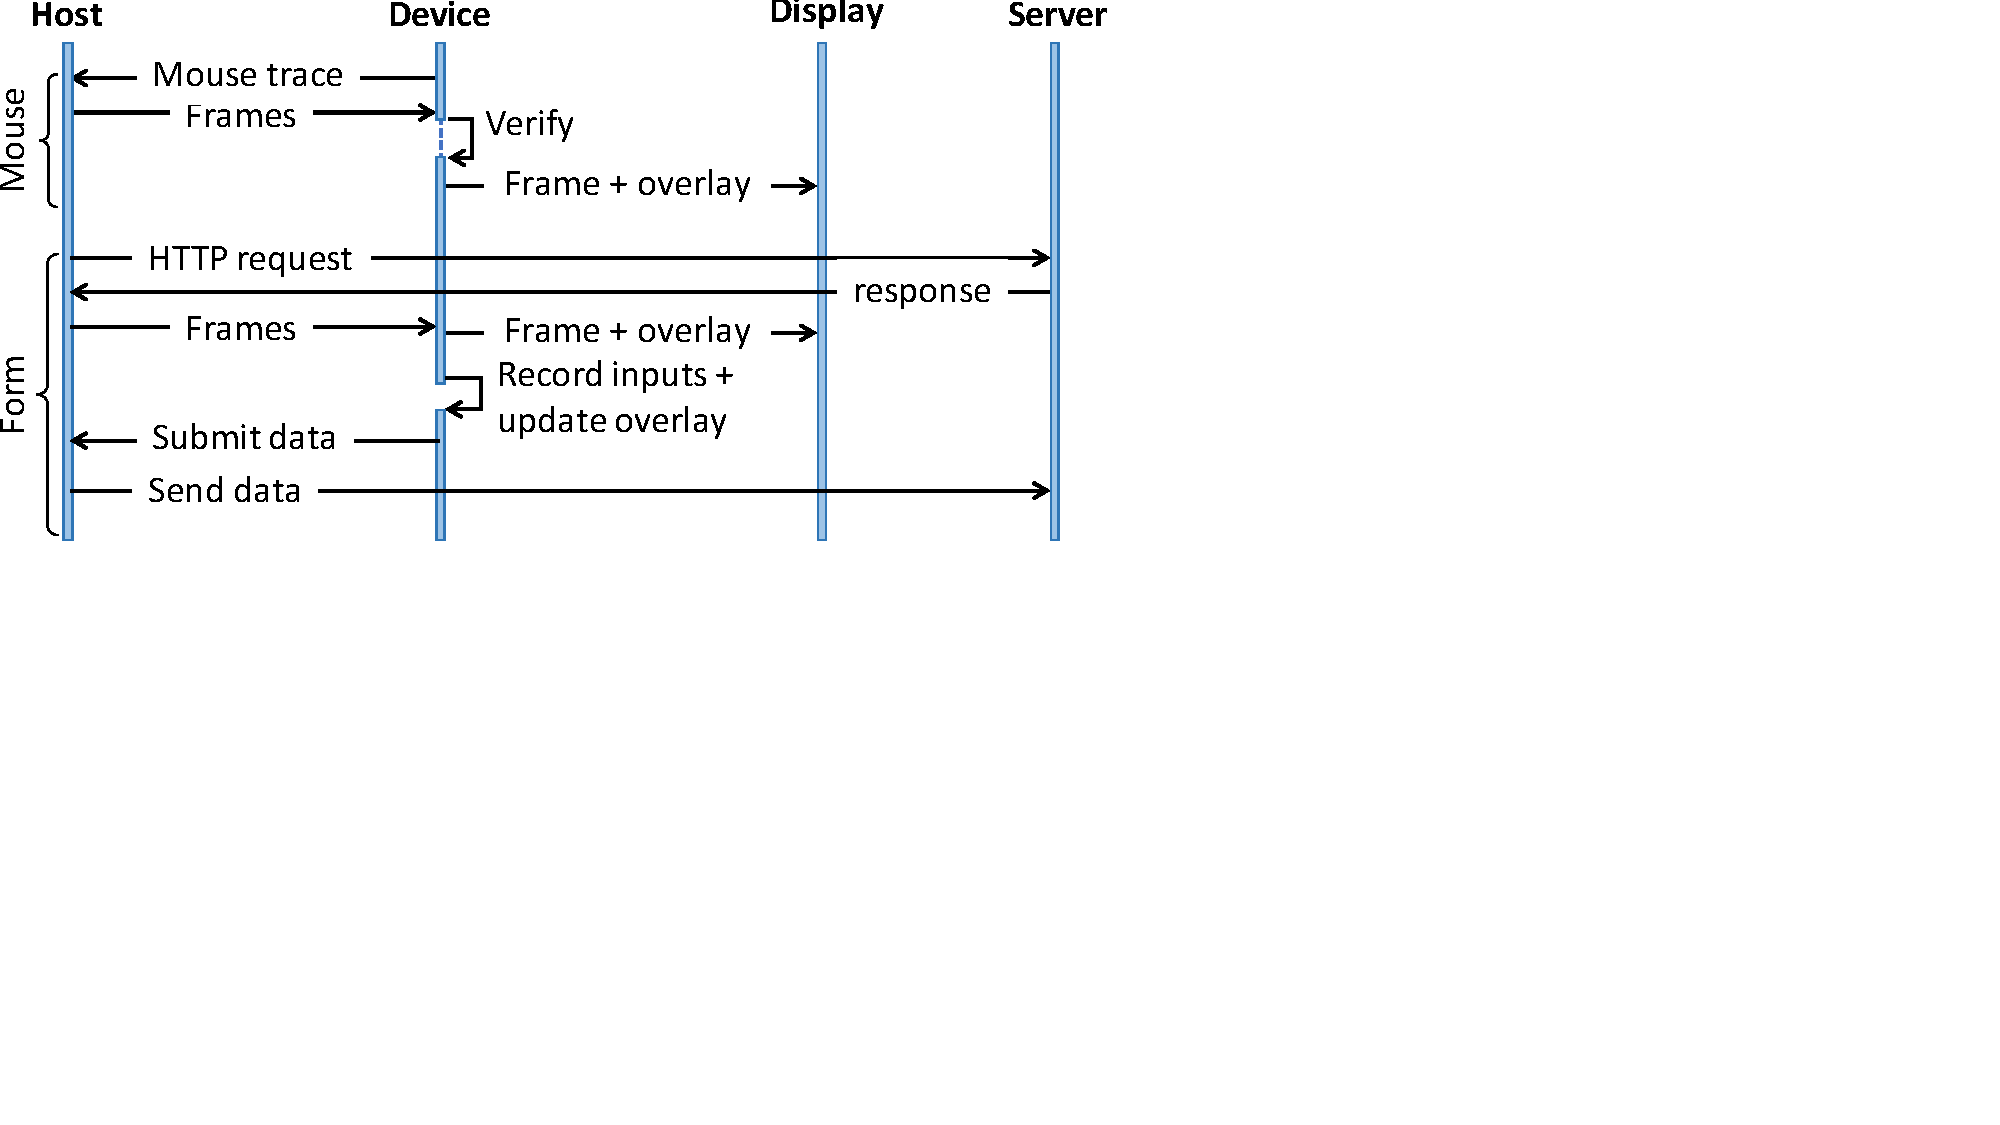
\includegraphics[trim={0 9.5cm 15cm 0}, clip, width=0.85\linewidth]{SequencDiagram.pdf}
\caption{\textbf{Flow of the \name main protocol.} The figure shows the
sequence of events for two example scenarios: mouse movement and filling up a
web-form.}
\spacesave
\label{fig:sequence}
\centering
\end{figure}


In the previous Sections, we explain the basic components of \name. Here we
summarize the overall flow of the system. The sequence diagram of \name is
illustrated in Figure~\ref{fig:sequence} that shows snapshots of two example
sequences: mouse movement and filling up a web-form.
%Now in this Section, we describe the flow of \name protocol by putting these
% components together. The outline of \name is illustrated in Figure~\ref{fig:sequence}. In the flow, we assume that the user already clicked on a web link or typed the URL in the address bar of the browser. This also allows the \device and the remote server to establish a \tls channel using the method described in Section~\ref{sec:confidentiality:tls}. The rest of the steps are as the following:

\iffalse
\begin{mylist}
  \item[\one] The browser renders the webpage that comes with \name JS. As described in Section~\ref{sec:systemDesign:transformation}, \name JS transforms the UI elements to a QR code that contains the equivalent UI specification.
  \item[\two] The graphics driver sends the rendered frame to the \device over the HDMI channel.
  \item[\three] The \device intercepts the HDMI signal and decode the QR code to retrieve the UI specification. After the decoding of the QR code, the \device renders the bitmap corresponding to the specification as described in Section~\ref{sec:systemDesign:transformation}.
  \item[\four] The \device send the HDMI frame with the UI overlay to the display device.
  \item[\five] After observing the HDMI frame and the overlaid UI, the user passes her input to the \device via the keyboard/mouse that is connected to the \device over the \usb interface.
  \item[\six] The \device uses raw mouse data and the HDMI frames to interpolate the mouse pointer using the method described in Section~\ref{sec:systemDesign:analysis}. This ensures pointer integrity. \device also overlays a mouse pointer on the HDMI frames.
  \item[\seven] When the user input her data to the host, the \device records her input data (Record phase in Section~\ref{sec:systemDesign:commit:send}).
  \item[\eight] The \name JavaScript snippet also acts as a upstream channel from the \device to the remote server (refer to Section~\ref{sec:systemDesign:commit:upload}). Via this channel, the \device sends the signed user action to the remote server. This signed user action can be seen as the second factor for the integrity of the user input data. (Commit phase in Section~\ref{sec:systemDesign:commit:send})
  \item [\nine] The server verifies the data from the two channels that are submitted by the host and the \device. (Section~\ref{sec:systemDesign:commit:verification})
\end{mylist}
\fi